\documentclass[a4paper]{article}
\usepackage[spanish]{babel}
\usepackage[utf8]{inputenc}
\usepackage[T1]{fontenc}
\usepackage{graphicx}

\title{Apuntes}
\author{Antonio Conde, Francisco Martínez, Ana Martínez}
\begin{document}
\maketitle

\section{Overleaf}
En PROJECT podemos seleccionar plantillas que tengamos en nuestro ordenador.

Para compartir el proyecto hay que pulsar en SHARE y copiar la dirección que nos aparece para enviarla por correo.

\section{Latex}
Hay unos botones en el encabezado que permiten introducir una Sección o una Subsección.

Otros niveles inferiores son \verb \subsubsection  y \verb \paragraph{} . Y niveles superiores son \verb \part{}  y \verb \chapter{} .

Si no queremos que una parte o sección no venga numerada ponemos un asterisco \verb \section*{} .

También hay botones para el tipo de letra negrita y cursiva. El resto de tipos se empieza con \verb \text ... Por ejemplo \textsc{En mayúsculas}

Tamaños de letra: normalsize, small, tiny,....

Para una cita textual:
\begin{quote}
Esta es una cita
\end{quote}

Para referenciar una sección, una tabla, una figura, etc, ponemos una label en dicho objeto y después lo referenciamos con ref.

Lista numerada con un botón dentro de More.
\begin{enumerate}
\item Primero
\item Segundo
\begin{enumerate}
\item Se pueden anidar listas
\item Utiliza letras
\end{enumerate}
\end{enumerate}

Lista no numerada
\begin{itemize}
\item Con circulo
\item Hay otras posibilidades
\end{itemize}

Vamos a dejar espacio
\vspace{1cm}

Comenzamos con las ecuaciones, primero con una ecuación en una línea: \(x_i\). Si queremos que la ecuación vaya numerada:
\[\bar{x} = \frac{\sum_{i=1}^n x_i}{n}\]

Introducimos una imagen. Lo primero es traer la imagen al proyecto. Para ello abrimos PROJECT y en files seleccionamos el archivo.
\begin{figure}[h!]
\centering
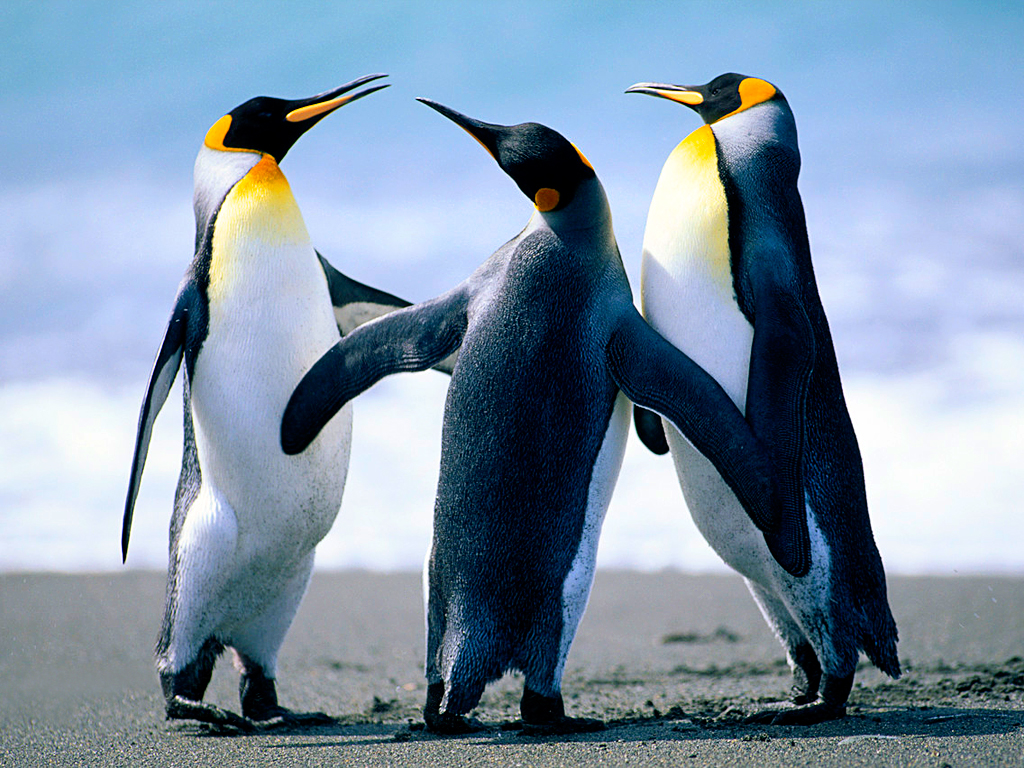
\includegraphics[width=5cm]{Penguins.jpg}
\caption{Fotografía de ping\"uinos}
\end{figure}
La admiración es para indicarle que es importante que tenga en cuenta la posición que le hemos dado (en este caso h es \textbf{here}).

\textbf{Nota}:  
Con la aplicación https//www.draw.io permite crear diagramas y grabarlos en formato vectorial (.pdf), para que sea del tamaño de la figura seleccionar: export -> pdf -> crop


\subsection{Referencias bibliográficas}

Podemos introducir un archivo .bib (a partir de files)

También podemos tener un gestor de referencias como Mendeley que trabaja en la web pero que también tiene una versión desktop. Una vez que estamos en Mendelay en library podemos instalar un complemento al navegador que permite introducir bibliografía muy cómodamente.

\bibliographystyle{abbrv}
\bibliography{MendeleyCurso}


\end{document}
